\documentclass[../TDE8_filtrage.tex]{subfiles}%

\begin{document}
\section[s]"2"{Filtre de \textsc{Colpitts}}

\enonce{%
	\noindent
	\begin{minipage}{.50\linewidth}
		On considère le quadripôle suivant, où $C$ est une capacité, $R$ une
		résistance et $L$ une inductance. Il est utilisé en régime sinusoïdal forcé
		de pulsation $\w$, en sortie «~ouverte~» (rien n'est branché aux bornes de
		sortie).
	\end{minipage}
	\begin{minipage}{0.50\linewidth}
		\begin{center}
			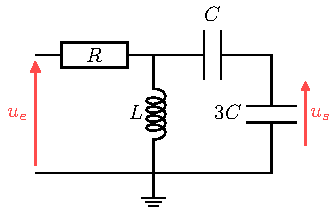
\includegraphics[width=.8\linewidth]{colpitts_plain}
		\end{center}
	\end{minipage}
}

\QR{%
	Étudier qualitativement le comportement de ce quadripôle en hautes et
	basses fréquences. De quel type de filtre s'agit-il~?
}{%
	~

	\vspace{-18pt}
	\begin{minipage}{0.48\linewidth}
		En basses fréquences ($\w \ra 0$), les condensateurs se
		comportent comme des interrupteurs ouverts, la bobine comme un fil~: la
		tension $u_s$ est donc nulle.
		\begin{center}
			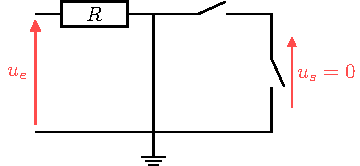
\includegraphics[width=\linewidth]{colpitts_bf}
		\end{center}
	\end{minipage}
	\hfill
	\vrule
	\hfill
	\begin{minipage}{0.48\linewidth}
		En hautes fréquences ($\w \ra \infty$), les condensateurs se
		comportent comme des fils, la bobine comme un interrupteur ouvert~: la
		tension $u_s$ est donc nulle.
		\begin{center}
			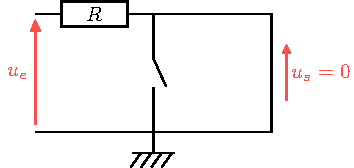
\includegraphics[width=\linewidth]{colpitts_hf}
		\end{center}
	\end{minipage}

	Comme la tension est nulle aux extrêmes, c'est un \textbf{passe-bande}.
	Si elle était égale à la tension d'entrée aux extrêmes, ça serait un
	coupe-bande.
}

\QR{%
	Déterminer la fonction de transfert $\Hu(\jw) =
		\dfrac{\xul{u_s}}{\xul{u_e}}$ et la mettre sous l'une des formes
	équivalentes~:
	\[\Hu(\jw) = \frac{A}{1+\jj Q \left( \dfrac{\w}{\w_0} -
			\dfrac{\w_0}{\w} \right)} = \frac{\jj\dfrac{A}{Q}\dfrac{\w}{\w_0}}{1
			- \dfrac{\w^2}{\w_0{}^2} + \dfrac{\jj}{Q} \dfrac{\w}{\w_0}}\]
	En introduisant des constantes $A$, $w_0$ et $Q$ dont on précisera les
	expressions en fonction de $R$, $L$ et $C$.
}{%
	On effectue deux diviseurs de tension successifs~: un pour déterminer
	$u_s$ en fonction de $u_L$, puis avec une impédance équivalente des
	trois dipôles de droite, on détermine $u_L$ en fonction de $u_e$ et on
	combine. C'est le même fonctionnement que pour l'exercice sur l'ADSL,
	question 3.
	\begin{center}
		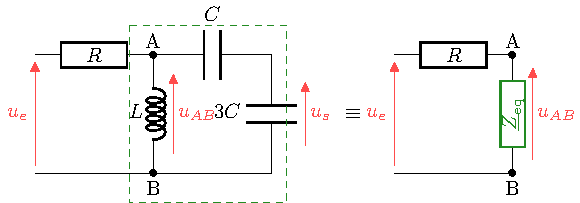
\includegraphics[width=0.8\linewidth]{colpitts_equiv}
	\end{center}
	On a ainsi en premier lieu
	\begin{gather*}
		\Uu_s = \frac{\Zu_{3C}}{\Zu_{3C} + \Zu_C}\Uu_{AB}
		\Lra
		\Uu_s = \frac{1/\jj3C\w}{1/\jj3C\w + 1/\jj C\w}\Uu_{AB}
		\Lra
		\Uu_s = \frac{1}{1+3}\Uu_{AB}
		\Lra
		\boxed{\Uu_s = \frac{\Uu_{AB}}{4}}
	\end{gather*}
	On aura donc ensuite~:
	\begin{gather*}
		\Uu_{AB} = \frac{\Zu\ind{eq}}{\Zu\ind{eq} + \Zu_R}\Uu_e
		\Lra
		\boxed{\Uu_{AB} = \frac{1}{1+\Zu_R\Yu\ind{eq}}\Uu_e}
	\end{gather*}
	On calcule alors $\Yu\ind{eq}$ de l'association en parallèle de $L$ et
	$C$ en série avec $3C$. \textbf{Attention} à l'association en série de
	capacités~:
	\begin{gather*}
		Z_{C+3C} = \frac{1}{\jj3C\w} + \frac{1}{\jcw}{\color{orange}\times
			\frac{3}{3}} = \frac{4}{\jj3C\w}\\
		\Yu\ind{eq} = \Yu_L + \Yu_{C+3C}
		\Lra
		\boxed{\Yu\ind{eq} = \frac{1}{\jlw} + \jj3C\w/4}
	\end{gather*}
	Et on combine~:
	\begin{gather*}
		\Uu_s =
		\frac{1}{4}
		\frac{1}{1+R \left( \dfrac{1}{\jlw} + \dfrac{\jj3C\w}{4} \right)}
		\Uu_e
		\Lra
		\Uu_s =
		\frac{1}{4}
		\frac{1}{1+\jj \left( - \dfrac{R}{L\w} + \dfrac{3RC\w}{4} \right)}
		\Uu_e
		\\
	\end{gather*}
	Ainsi, en divisant par $\Uu_e$ pour avoir la fonction de transfert, on
	a~:
	\begin{gather*}
		\Hu = \frac{1/4} {1+\jj\left(\dfrac{3RC\w}{4}-\dfrac{R}{L\w}\right)}
		\Lra
		\boxed{\Hu = \frac{A}{1+\jj Q \left( \dfrac{\w}{\w_0} -
				\dfrac{\w_0}{\w} \right)}}
		\qavec
		\boxed{A = \frac{1}{4}}
	\end{gather*}
	Reste à trouver $Q$ et $\w_0$. Pour cela, on identifie membre à membre~:
	\begin{align*}
		\frac{Q}{\w_0} = \frac{3RC}{4} \quad (1)
		 & \qet
		Q\w_0 = \frac{R}{L} \quad (2) \\
		\Lra
		\boxed{Q = \frac{R\sqrt{3C}}{2\sqrt{L}}}
		 & \qet
		\boxed{\w_0 = \frac{2}{\sqrt{3LC}}}
	\end{align*}
	où l'on obtient $Q$ et $\w_0$ en multipliant les équations (1) et (2)
	d'une part puis en en prenant la racine carrée, et en divisant (2) par
	(1) en en prenant la racine carrée, respectivement.
}
\enonce{%
	Le diagramme de \textsc{Bode} de ce quadripôle pour $Q = 6$ est donné
	ci-dessous.
	\begin{center}
		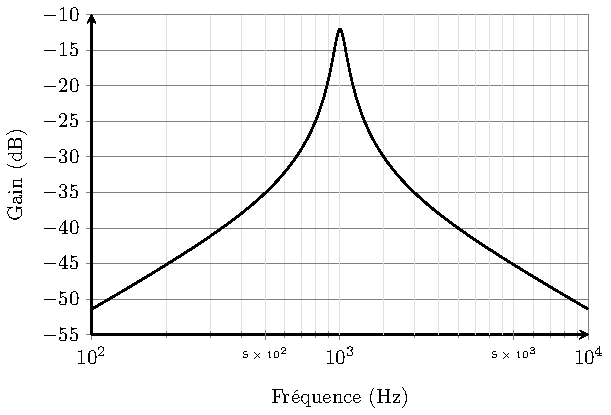
\includegraphics[width=.46\linewidth]{colpitts_bode-gain}
		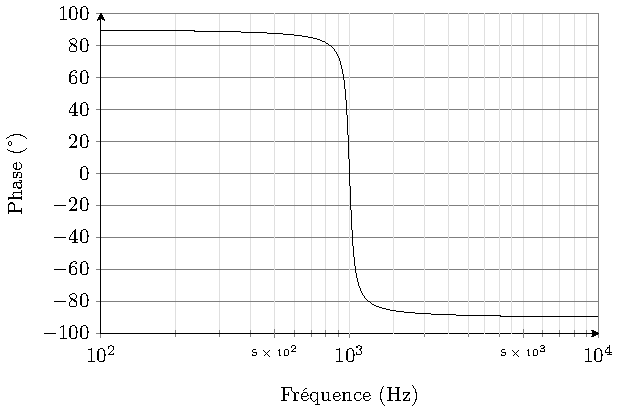
\includegraphics[width=.46\linewidth]{colpitts_bode-phase}
	\end{center}
}

\QR{%
	Justifier l'allure des parties rectilignes du diagramme.
	Déduire du diagramme la valeur de la fréquence d'accord $f_0 =
		\w_0/2\pi$ ainsi que des fréquences de coupure.
}{%
	Les parties rectilignes du diagramme correspondent aux limites
	asymptotiques du gain en décibels, c'est-à-dire pour $\w \ll \w_0$ et
	$\w \gg \w_0$. En effet,
	\begin{align*}
		\Hu \underset{\w \ll \w_0}{\sim} \jj \frac{A}{Q} \frac{\w}{\w_0}
		 & \qet
		\Hu \underset{\w \gg \w_0}{\sim} -\jj \frac{A}{Q} \frac{\w_0}{\w}
		\\
		\Lra
		G_{\dB} \underset{\w \ll \w_0}{\sim}
		20 \log \frac{A}{Q} + 20 \log \frac{\w}{\w_0}
		 & \qet
		G_{\dB} \underset{\w \gg \w_0}{\sim}
		20 \log \frac{A}{Q} - 20 \log \frac{\w}{\w_0}
		\\
		\Lra
		\f \underset{\w \ll \w_0}{\sim} \frac{\pi}{2}
		 & \qet
		\f \underset{\w \gg \w_0}{\sim} - \frac{\pi}{2}
	\end{align*}
	Pour $\w = \w_0$, on trouve simplement $\Hu = A$ donc $G_{\dB}(\w_0) =
		\SI{-12}{dB}$ et $\f = 0$. La fréquence de résonance (ou fréquence d'accord)
	correspond au pic du diagramme de \textsc{Bode} (ou à l'intersection des
	asymptotes du gain en décibels) d'une part, ou correspond à la fréquence
	pour laquelle la phase est nulle~: on lit simplement \fbox{$f_0 =
			\SI{1}{kHz}$}. \bigbreak
	On trouve les fréquences de coupure en trouvant les fréquences $f_1$ et
	$f_2$ telles que $G_{\dB} = G_{\max} - \SI{3}{dB}$, soit $G_{\dB} =
		\SI{-15}{dB}$~: on lit approximativement \fbox{$f_1 = \SI{950}{Hz}$} et
	\fbox{$f_2 = \SI{1050}{Hz}$}.
}

\end{document}
